\documentclass{article}

\usepackage[letterpaper,top=2cm,bottom=2cm,left=3cm,right=3cm,marginparwidth=1.75cm]{geometry}
\usepackage{algorithm2e}

% Useful packages
\usepackage{amsmath}
\usepackage{graphicx}
\usepackage[colorlinks=true, allcolors=blue]{hyperref}
\usepackage{hyperref}

\title{Spooky House}
\author{Jamie Wales}

\begin{document}
    \maketitle


    \section{Overview}\label{sec:introduction}

    \subsection{Core Concept}
    "Spooky House" is a high-octane first-person shooter that combines the wave-based survival mechanics of Call of Duty Zombies, the fast-paced arena combat of Quake/Doom, and the bullet-time manipulation from The Matrix (PS2). Players battle against increasingly difficult waves of enemies while utilising superhuman reflexes to slow down time, perform impossible stunts, and eliminate threats with stylish precision.

    \subsection{Genre}
    "Spooky House" is first and foremost a first-person shooter. However, it combines the following sub-genres to create a unique and engaging experience:
    \begin{itemize}
        \item First-Person Shooter
        \item Survival Horror
        \item Bullet-Time Action
        \item Arena Combat
    \end{itemize}

    \subsection{Insperation}
    Here is an overview of games that has inspired "Spooky House"'s core mechanics and design

    \subsubsection{Call of Duty Zombies}
    Call of Duty Zombies is a wave-based survival mode that has become a staple of the franchise.
    Players must survive against increasingly difficult waves of enemies while utilising the environment and special weapons to stay alive.
    Spooky House takes inspiration from this mode by incorporating wave-based survival mechanics.
    As the game progresses the player will have access to increasingly powerful weapons and abilities to help them survive.
    The game will not implement the room-based system of Call of Duty Zombies, instead opting for a more open-world approach.
    Weapons will drop off of enemies, making it important to kill as many enemies as possible to get the best weapons.

    \subsubsection{Doom/Quake}
    Doom and Quake are fast-paced arena shooters that focus on movement and precision shooting.
    Players must navigate complex levels while battling against hordes of enemies.
    The movement system will directly integrate with score and the bullet time mechanic.
    Players will receive more points for killing enemies in stylish ways, such as headshots, while in bullet time or whilst moving.
    The game will also feature a combo system that rewards players for chaining together kills and stunts.
    The player's bullet time meter will increase with more stylish kills and movement, encouraging players to play aggressively and take risks, and giving them a satisfying core loop of killing enemies, gaining points, and using those points to gain more bullet time.

    \subsubsection{The Matrix (PS2)}
    The Matrix video game for PS2 featured a bullet time mechanic that allowed players to slow down time and perform impossible stunts.
    This mechanic will be a core feature of Spooky House, allowing players to slow down time to dodge bullets, perform acrobatic moves, and eliminate enemies with precision.
    The bullet time mechanic will be tied to a meter that depletes as the player uses it, encouraging strategic use of the ability.
    Spooky house will also feature a "focus" mechanic that allows players to slow down time even further for a short period, allowing them to perform even more impressive stunts and kills.
    The game will encourage use of this feature, allowing players to turn on and off bullet time at will, and rewarding them for using it in creative ways.

    \subsubsection{Devil May Cry}
    Devil May Cry is a action game that rewards players for performing stylish combos and kills.
    Spooky house will implement a style based score system after each wave encouraging reliability and mastery of the game.
    The game will also feature a variety of weapons and abilities that players can use to customise their play style and create unique combos.
    The game will also feature a variety of enemies with different weaknesses and attack patterns, encouraging players to adapt their playstyle and strategy to overcome each wave.

    \subsection{Target Audience}
    \begin{itemize}
        \item FPS enthusiasts aged 18-35 who enjoy fast-paced shooters with unique mechanics
        \item Fans of classic gaming, particularly those with nostalgia for PlayStation 2 era aesthetics
        \item Action game players looking for stylish combat with high skill expression
    \end{itemize}

    \subsection{Unique Selling Points}
    \begin{itemize}
        \item Bullet Time: Slow down time while maintaining movement speed, allowing for spectacular dodges, precision aiming, and cinematic moments
        \item Wave Escalation: Survive increasingly difficult waves of enemies with intermittent boss encounters
        \item Movement Mechanics: Utilise double jumps, wall runs, and slides that become even more powerful during bullet time
        \item Kill Combos: Chain kills to build momentum, unlock special abilities, and earn score multipliers
    \end{itemize}


    \section{Work complete}
    A lot of the current work has gone into systems which the game can built built on top of. A great deal of effort has gone into using scriptable objects to hold the data in which the systems rely.
    This way, the game can be easily expanded upon and changed without having to change the code. This is a great way to work as it allows for a lot of flexibility and creativity in the development process.
    This section will explain what features have been built thus far.

    \subsection{Player Movement}
    This is a cornerstone of the Spooky House experience, serving as the foundation upon which all other gameplay elements are built. Drawing inspiration from arena shooters like Quake and Doom, the movement system emphasizes speed, fluidity, and acrobatic potential.

    \subsubsection{Player Animation States}
    The player character utilizes a state-based animation system with smooth transitions between key states. Figure \ref{fig:player-states} shows the primary animation states and their transitions.
    The animation system uses boolean parameters and triggers in the Unity Animator to control transitions between states. The core animation states are:
    \begin{itemize}
        \item \textbf{Idle}: Default state when no input is detected
        \item \textbf{Run}: Active when movement input is detected
        \item \textbf{Shoot}: Triggered by left mouse button
        \item \textbf{Reload}: Activated by pressing R key
        \item \textbf{Jump/Dive}: Special movement states with jump triggered by space bar, and dive by pressing space again during the jump window
    \end{itemize}
    The dive roll mechanic provides both gameplay advantages (brief invulnerability) and scoring benefits (increased style multiplier).

    \subsubsection{Core Movement Implementation}
    The current implementation features a robust character controller that provides dynamic movement options (dive roll algorithm detailed in Appendix \ref{appendix:player-movement}):
    \begin{itemize}
        \item Variable movement speeds (walking and sprinting) with smooth transitions
        \item Precision jumping mechanics with adjustable force parameters
        \item Advanced double-jump capabilities with a timing window
        \item Signature dive roll maneuver for evasive action and stylish combat
        \item Custom ground detection using raycasting for improved responsiveness
        \item Full animation integration with state transitions
    \end{itemize}
    The dive roll mechanic is particularly significant as it represents a key element of the movement system. When a player jumps and then presses jump again within the double-jump time window, they execute a forward dive that can be used to dodge incoming fire, close distance to enemies, or position for spectacular kills that earn style points.

    \subsubsection{Technical Challenges Overcome}
    Developing this movement system presented several technical challenges that have been successfully addressed:
    \begin{itemize}
        \item Creating reliable ground detection that works with complex geometry
        \item Implementing smooth transitions between movement states
        \item Ensuring dive roll momentum and direction feel natural and responsive
        \item Balancing movement speeds and jump forces for satisfying gameplay
    \end{itemize}

    The current system uses a combination of character controller methods and custom physics calculations to achieve smooth, responsive movement that maintains player control even during complex maneuvers.
    The implementation carefully monitors the player's grounded state, handles input for different movement types, and manages the specialized dive roll functionality.
    The dive roll implementation required particular attention to detail, as it needed to determine appropriate direction based on either the player's current velocity or input direction.
    This ensures that players can execute stylish dives in any direction they choose, adding both tactical options and visual flair to combat scenarios.

    \subsection{Enemy System}
    The enemy system in "Spooky House" forms the cornerstone of the combat experience, providing dynamic and responsive opponents that challenge the player's skills.
    The implementation uses a robust state machine architecture that allows enemies to react intelligently to the player's actions.

    \subsubsection{State-Based AI}
    Enemies operate on a sophisticated state machine that transitions between six distinct behavioral states (see Appendix \ref{appendix:enemy-ai} for the full algorithm implementation):

    \begin{itemize}
        \item \textbf{Idle}: The default state where enemies remain stationary while scanning for the player
        \item \textbf{Patrol}: Enemies navigate randomly through the environment using Unity's NavMesh system
        \item \textbf{Chase}: Upon detecting the player, enemies actively pursue using pathfinding
        \item \textbf{Attack}: Within range, enemies execute attacks with appropriate animations and effects
        \item \textbf{Hurt}: A transitional state triggered when enemies take damage
        \item \textbf{Dead}: Handles death animations, particle effects, and eventual removal from the scene
    \end{itemize}

    This state-based approach allows enemies to make contextual decisions based on player proximity, previous actions, and environmental factors. Each state has its own specific behaviors and transition conditions, creating emergent gameplay scenarios as enemies respond dynamically to the player's tactics.

    \subsubsection{NavMesh Integration}
    The enemy movement system leverages Unity's NavMesh for intelligent pathfinding, allowing enemies to navigate complex environments while pursuing the player. Key features include:

    \begin{itemize}
        \item Dynamic path calculation to track moving targets
        \item Stuck detection and recovery mechanisms
        \item Speed variations between patrol and chase states
        \item Variable stopping distances based on attack ranges
    \end{itemize}

    This integration ensures enemies can navigate realistically around obstacles while maintaining pursuit pressure on the player, regardless of the arena's complexity.

    \subsubsection{Scriptable Object Architecture}
    Enemy behaviors and attributes are defined through a flexible scriptable object system (EnemyData) that decouples data from implementation. This approach allows for:

    \begin{itemize}
        \item Easy creation of diverse enemy types without code changes
        \item Centralized balancing of health, damage, and speed values
        \item Assignment of custom animations, sounds, and visual effects
        \item Runtime variation of enemy capabilities
    \end{itemize}

    This data-driven design enables rapid iteration and easy expansion of the enemy roster, supporting the game's wave-based progression system.

    \subsubsection{Combat Feedback Systems}
    Enemies provide rich feedback during combat encounters through:

    \begin{itemize}
        \item Visual hit reactions and knockback effects
        \item Contextual audio cues for different states
        \item Particle effects for hits and death sequences
        \item Animation transitions that reflect current behavior
    \end{itemize}

    These feedback mechanisms communicate the game state clearly to the player while enhancing the satisfaction of combat encounters.

    \subsubsection{Technical Resilience}
    The enemy system includes numerous safeguards to ensure stable operation even under edge cases:

    \begin{itemize}
        \item Component verification with automatic addition of missing requirements
        \item NavMesh position validation to prevent navigation errors
        \item Error-resistant animation handling with exception management
        \item Graceful destruction sequence to prevent runtime errors
    \end{itemize}

    \subsection{Wave Spawning System}
    The Wave Spawning System in "Spooky House" drives the game's core progression mechanics, creating an escalating challenge through procedurally generated enemy waves. This system implements the survival foundation inspired by Call of Duty Zombies while adapting it to the more open, arena-based environment.

    \subsubsection{Dynamic Wave Generation}
    The spawning system creates waves with increasing difficulty through procedural generation (algorithm provided in Appendix \ref{appendix:wave-spawning}):

    \begin{itemize}
        \item Configurable enemy count ranges that can scale with wave progression
        \item Randomized spawn locations within a defined radius around spawn points
        \item NavMesh validation to ensure enemies spawn on valid traversable surfaces
        \item Timed intervals between enemy spawns to create manageable combat pacing
        \item Cooldown periods between waves to allow players recovery time
    \end{itemize}

    This approach creates unpredictable but fair combat scenarios, ensuring each playthrough feels fresh while maintaining a consistent difficulty curve.

    \subsubsection{Enemy Type Selection}
    The system leverages the scriptable object architecture to create diverse enemy compositions:

    \begin{itemize}
        \item Waves draw from a configurable pool of enemy types
        \item Random selection ensures varied combat encounters
        \item Enemy data is passed to spawned instances, controlling their behavior and capabilities
        \item Each enemy is named contextually based on wave number and remaining count for debugging
    \end{itemize}

    This implementation allows for easy expansion of the enemy roster and supports natural difficulty progression as more challenging enemy types can be introduced in later waves.

    \subsubsection{Wave Management}
    The system maintains complete awareness of the current game state through:

    \begin{itemize}
        \item Active tracking of all spawned enemies
        \item Automatic cleanup of destroyed enemies
        \item Wave completion detection when all enemies are defeated
        \item Wave progression counters for scaling difficulty
    \end{itemize}

    This creates a rhythm of combat intensity and brief respite that forms the core gameplay loop of "Spooky House," pushing players to survive increasingly challenging scenarios while providing moments to recover between waves.

    \subsubsection{Technical Implementation}
    The spawning system integrates with other game systems through:

    \begin{itemize}
        \item Direct configuration of spawned enemy controllers
        \item Player reference passing to ensure enemies can locate their target
        \item Unity's NavMesh system for spawn position validation
        \item Coroutine-based spawning for controlled timing
    \end{itemize}

    The system uses a combination of Update cycle checks and coroutines to manage wave timing, enemy spawning, and cleanup operations efficiently. This hybrid approach ensures responsive wave management without creating performance bottlenecks during intense combat.

    \subsection{Weapon System}
    The weapon system in "Spooky House" provides players with diverse and satisfying combat options. Built on scriptable objects for maximum flexibility, the system supports a variety of weapon types that can be collected and cycled through during gameplay.

    \subsubsection{Weapon Management}
    The core weapon management features include:

    \begin{itemize}
        \item Automatic weapon attachment to the player character's hand bone
        \item Cycling between multiple weapon types during gameplay
        \item Configurable positioning, rotation, and scale for each weapon
        \item Weapon-specific parameters including damage, fire rate, and ammunition capacity
        \item Animation integration with the player character's animation controller
    \end{itemize}

    This flexibility allows for a wide range of weapon types that each feel distinct while maintaining a coherent attachment to the player model. The system uses Unity's humanoid animation rigging to automatically locate and attach weapons to the player's hand.

    \subsubsection{Visual Feedback}
    Combat feedback is critical to creating satisfying gunplay, and the weapon system provides rich visual cues:

    \begin{itemize}
        \item Muzzle flash effects using Unity's Visual Effect Graph system
        \item Bullet trail renderers with object pooling for performance
        \item Dynamic movement of trails along calculated bullet paths
        \item Custom crosshair expansion to indicate weapon firing
        \item Animation triggers for player shooting and reloading actions
    \end{itemize}

    Object pooling for bullet trails ensures that even during high-intensity combat with multiple rapid-fire weapons, performance remains smooth with minimal garbage collection overhead.

    \subsubsection{Weapon Data Architecture}
    The scriptable object-based weapon data system allows for:

    \begin{itemize}
        \item Easy creation and balancing of new weapon types
        \item Centralized management of weapon properties
        \item Runtime ammunition tracking
        \item Weapon-specific audio and visual effects
    \end{itemize}

    This data-driven approach streamlines the creation process for new weapons and facilitates rapid prototyping and balancing.

    \subsection{Bullet Time System}
    The bullet time mechanic represents one of "Spooky House's" most distinctive features, offering players superhuman reflexes inspired by "The Matrix" video game. This system creates dramatic slow-motion sequences while maintaining player agency and control.

    \subsubsection{Time Manipulation}
    The core of the bullet time system involves carefully managed time dilation (detailed in Appendix \ref{appendix:bullet-time}):

    \begin{itemize}
        \item Adjustable time scale with configurable slowdown factor (currently 0.3x normal speed)
        \item Preservation of physics consistency through fixedDeltaTime adjustments
        \item Energy resource management to limit usage
        \item Automatic deactivation when energy is depleted
        \item Gradual energy recharge when not in use
    \end{itemize}

    This creates a tactical resource that players must manage, encouraging strategic activation during key moments rather than constant use.

    \subsubsection{Audiovisual Effects}
    To enhance the bullet time experience, the system implements comprehensive audiovisual changes:

    \begin{itemize}
        \item Screen tinting with configurable color to indicate the active state
        \item Global audio adjustments including volume reduction and pitch shifting
        \item Dedicated bullet time activation sound that plays at normal speed
        \item State restoration when bullet time ends
    \end{itemize}

    These effects create a dramatic shift in the game's presentation when bullet time is active, enhancing the sensation of heightened reflexes and perception.

    \subsubsection{Implementation Approach}
    The bullet time system uses several technical approaches to ensure smooth operation:

    \begin{itemize}
        \item Singleton pattern for global access from other systems
        \item Dictionary tracking of all audio sources for consistent sound management
        \item Unscaled time for energy depletion to ensure consistent drain rate
        \item Dynamically created UI elements for visual feedback
    \end{itemize}

    The system also includes safeguards to ensure time scale is always properly restored when the player exits bullet time, preventing potential game-breaking states where time remains permanently slowed.
    \appendix


    \section{Technical Algorithms}
    \label{appendix:algorithms}

    This appendix contains the pseudocode implementations of key algorithms that power the core mechanics of "Spooky House."

    \newpage

    \subsection{Enemy AI State Machine}
    \label{appendix:enemy-ai}

    The following algorithm demonstrates the state-based decision making that drives enemy behavior in the game:

    \begin{algorithm}[H]
        \SetAlgoLined
        \KwResult{Updated enemy state and behavior}
        \While{enemy is alive}{
            currentState = GetCurrentState()\;
            \Switch{currentState}{
                \Case{IDLE}{
                    UpdateAnimationState(false, false)\;
                    agent.isStopped = true\;
                    waitTimer += Time.deltaTime\;
                    \If{waitTimer > randomIdleTime}{
                        \If{canPatrol}{
                            SetState(PATROL)\;
                        }
                    }
                    \If{DistanceToPlayer() < detectionRadius}{
                        SetState(CHASE)\;
                    }
                }
                \Case{PATROL}{
                    UpdateAnimationState(true, false)\;
                    agent.isStopped = false\;
                    \If{!hasDestination}{
                        destination = GetRandomNavMeshPoint(position, patrolRadius)\;
                        agent.SetDestination(destination)\;
                    }
                    \If{ReachedDestination()}{
                        SetState(IDLE)\;
                    }
                    \If{DistanceToPlayer() < detectionRadius}{
                        SetState(CHASE)\;
                    }
                }
                \Case{CHASE}{
                    UpdateAnimationState(true, true)\;
                    agent.isStopped = false\;
                    agent.SetDestination(playerPosition)\;
                    \If{DistanceToPlayer() <= attackRange}{
                        SetState(ATTACK)\;
                    }
                    \If{DistanceToPlayer() > losePlayerRadius}{
                        SetState(IDLE)\;
                    }
                }
                \Case{ATTACK}{
                    UpdateAnimationState(false, false)\;
                    agent.isStopped = true\;
                    FaceTarget(playerPosition)\;
                    \If{Time.time - lastAttackTime > attackCooldown}{
                        PerformAttackSequence()\;
                        lastAttackTime = Time.time\;
                    }
                    \If{DistanceToPlayer() > attackRange * 1.1}{
                        SetState(CHASE)\;
                    }
                }
            }
        }
        \caption{Enemy State Machine Algorithm}
    \end{algorithm}

    The algorithm implements a state machine controlling enemy behavior. Enemies transition between idle, patrol, chase, and attack states based on player proximity and timers. Each state has specific behaviors, like randomly patrolling when idle or attacking when the player is within range. The system integrates with Unity's NavMesh for pathfinding, enabling enemies to navigate complex environments while pursuing the player.

    \newpage

    \subsection{Bullet Time System}
    \label{appendix:bullet-time}

    The signature bullet time feature is implemented through the following algorithm which carefully manages time scale, player physics, and environmental effects:

    \begin{algorithm}[H]
        \SetAlgoLined
        \KwResult{Modified time scale with preserved player physics}
        \SetKwFunction{FMain}{ToggleBulletTime}
        \SetKwProg{Fn}{Function}{:}{}
        \Fn{\FMain{bool activate}}{
            \If{activate \AND currentEnergy > 0}{
                originalTimeScale = Time.timeScale\;
                Time.timeScale = bulletTimeScale\;
                Time.fixedDeltaTime = defaultFixedDeltaTime * Time.timeScale\;
                isInBulletTime = true\;

                PlayBulletTimeAudio()\;
                AdjustAllEnvironmentalSounds(loweredVolume, loweredPitch)\;
                ActivateVisualEffect(screenTint)\;

                // Apply player-specific physics preservation
                playerController.moveSpeed *= (1 / bulletTimeScale)\;
                playerController.jumpForce *= (1 / bulletTimeScale)\;
            }
            \Else{
                Time.timeScale = 1.0f\;
                Time.fixedDeltaTime = defaultFixedDeltaTime\;
                isInBulletTime = false\;

                StopBulletTimeAudio()\;
                RestoreAllEnvironmentalSounds()\;
                DeactivateVisualEffect(screenTint)\;

                // Restore normal player physics
                playerController.moveSpeed = defaultMoveSpeed\;
                playerController.jumpForce = defaultJumpForce\;
            }
        }
        \caption{Bullet Time Toggle Algorithm}
    \end{algorithm}

    This algorithm manages the game's signature bullet time mechanic. When activated (and if sufficient energy is available), it slows down the game's time scale while preserving the player's relative movement speed. The system adjusts audio (lowering volume and pitch of environmental sounds), applies visual effects (screen tinting), and modifies physics parameters to maintain responsive player control. When deactivated, all parameters are restored to normal values.

    \newpage

    \subsection{Wave Spawning System}
    \label{appendix:wave-spawning}

    Enemy waves are dynamically generated using the following algorithm that scales difficulty based on player progression:

    \begin{algorithm}[H]
        \SetAlgoLined
        \KwResult{Progressive enemy spawning with difficulty scaling}
        \SetKwFunction{FMain}{SpawnWave}
        \SetKwProg{Fn}{Function}{:}{}
        \Fn{\FMain{int waveNumber}}{
            isSpawning = true\;

            // Calculate wave parameters with progressive difficulty
            baseEnemyCount = minEnemiesPerWave + (waveNumber * 0.5)\;
            enemyCount = min(baseEnemyCount, maxEnemiesPerWave)\;
            remainingEnemies = enemyCount\;

            // Calculate enemy type distribution
            standardEnemyChance = max(0.9 - (waveNumber * 0.05), 0.4)\;
            specialEnemyChance = 1.0 - standardEnemyChance\;

            // Determine if boss wave
            isBossWave = (waveNumber \% 5 == 0) \AND (waveNumber > 0)\;

            \If{isBossWave}{
                SpawnBossEnemy()\;
                remainingEnemies += 1\;
            }

            // Spawn regular enemies
            \For{i = 0 \KwTo enemyCount - 1}{
                spawnPosition = GetValidSpawnPosition()\;
                enemyType = DetermineEnemyType(standardEnemyChance, specialEnemyChance)\;
                SpawnEnemy(enemyType, spawnPosition)\;
                yield WaitForSeconds(spawnInterval)\;
            }

            isSpawning = false\;
            nextWaveTime = Time.time + timeBetweenWaves\;
        }
        \caption{Dynamic Wave Spawning Algorithm}
    \end{algorithm}

    This algorithm controls the game's wave-based enemy spawning system. It dynamically scales difficulty by increasing enemy numbers as waves progress and adjusting the likelihood of encountering special enemy types. Every fifth wave triggers a boss encounter for added challenge. The system ensures proper spacing between enemy spawns and validates spawn positions against the NavMesh to prevent enemies from appearing in invalid locations.

    \newpage

    \subsection{Player Movement System}
    \label{appendix:player-movement}

    The player's acrobatic movement capabilities, including the signature dive roll, are implemented as follows:

    \begin{algorithm}[H]
        \SetAlgoLined
        \KwResult{Player movement with dive roll capabilities}
        \SetKwFunction{FMain}{HandleJumpAndDive}
        \SetKwProg{Fn}{Function}{:}{}
        \Fn{\FMain{}}{
            jumpButtonPressed = Input.GetButtonDown("Jump")\;

            \If{jumpButtonPressed}{
                \If{isGrounded}{
                    // First jump
                    velocity.y = jumpForce\;
                    canDive = true\;
                    lastJumpTime = Time.time\;
                    PlayAnimation("jump")\;
                }
                \ElseIf{canDive \AND (Time.time - lastJumpTime < doubleJumpWindow)}{
                    // Dive roll on second press within window
                    ExecuteDiveRoll()\;
                }
            }
        }

        \SetKwFunction{FRoll}{ExecuteDiveRoll}
        \SetKwProg{Fn}{Function}{:}{}
        \Fn{\FRoll{}}{
            // Determine dive direction
            horizontalVelocity = new Vector3(controller.velocity.x, 0, controller.velocity.z)\;

            \If{horizontalVelocity.magnitude > 0.5}{
                diveDirection = horizontalVelocity.normalized\;
            }
            \Else{
                diveDirection = GetInputDirection()\;

                \If{diveDirection.magnitude < 0.1}{
                    diveDirection = transform.forward\;
                }
            }

            // Apply vertical boost
            velocity.y = jumpForce * 0.5\;

            // Start animation
            PlayAnimation("diveRoll")\;

            isDiving = true\;
            canDive = false\;

            // During fixed update, apply:
            // controller.Move(diveDirection * (diveForce * Time.deltaTime))
        }
        \caption{Player Dive Roll System Algorithm}
    \end{algorithm}

    This algorithm manages the player's movement system, with particular focus on the signature dive roll mechanic. The system tracks the player's grounded state using raycasting for precision. When the jump button is pressed while grounded, the player executes a standard jump and starts a time window for dive roll eligibility. If the jump button is pressed again within this window, the player performs a dive roll in the direction of current movement or input. The dive roll provides both tactical advantages (evasion, positioning) and scoring benefits.

    \newpage

    \subsection{Combat Scoring System}
    \label{appendix:scoring}

    The stylish combat scoring system evaluates player actions and assigns points based on the following algorithm:

    \begin{algorithm}[H]
        \SetAlgoLined
        \KwResult{Combat style score with multipliers}
        \SetKwFunction{FMain}{EvaluateKillStyle}
        \SetKwProg{Fn}{Function}{:}{}
        \Fn{\FMain{Enemy enemy, DamageInfo damageInfo}}{
            baseScore = 100\;
            styleMultiplier = 1.0\;

            // Time since last kill affects combo
            timeSinceLastKill = Time.time - lastKillTime\;

            // Base multipliers
            \If{damageInfo.isHeadshot}{
                styleMultiplier += 0.5\;
            }

            \If{player.isInBulletTime}{
                styleMultiplier += 0.3\;
            }

            \If{player.isDiving}{
                styleMultiplier += 0.6\;
            }

            \If{player.isInAir}{
                styleMultiplier += 0.4\;
            }

            // Combo multiplier
            \If{timeSinceLastKill < comboTimeWindow}{
                killCombo += 1\;
                comboMultiplier = min(1.0 + (killCombo * 0.1), 3.0)\;
            }
            \Else{
                killCombo = 0\;
                comboMultiplier = 1.0\;
            }

            // Distance bonus
            distanceToEnemy = Vector3.Distance(player.position, enemy.position)\;
            distanceMultiplier = 1.0 + (distanceToEnemy / 50.0)\; // Max 1.5x at 25m

            // Calculate final score
            finalScore = baseScore * styleMultiplier * comboMultiplier * distanceMultiplier\;

            // Update player state
            totalScore += finalScore\;
            lastKillTime = Time.time\;

            // Reward bullet time energy
            bulletTimeEnergy += finalScore * 0.05\;

            // Display style text
            DisplayStyleText(DetermineStyleRank(styleMultiplier))\;

            return finalScore\;
        }
        \caption{Style-Based Combat Scoring Algorithm}
    \end{algorithm}

    This algorithm implements the game's style-based scoring system, inspired by Devil May Cry's combo mechanics. It evaluates kills based on multiple factors: execution method (headshots), player state (in bullet time, diving, airborne), combo timing, and distance from target. Players are rewarded for chaining kills quickly with an escalating combo multiplier that can reach up to 3x. The system also incentivizes risk-taking by awarding higher scores for kills performed at greater distances. As a gameplay loop reinforcement, a portion of the score earned is converted to bullet time energy, encouraging players to perform stylish kills to maintain their bullet time capabilities.

    \newpage

    \subsection{Characters}
    \begin{figure}[h]
        \centering
        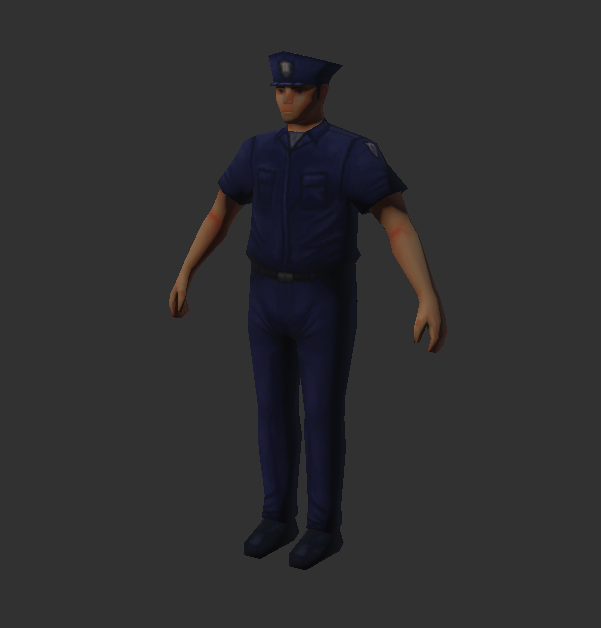
\includegraphics[width=0.8\textwidth]{Officer Edwards.png}
        \caption{Officer Edwards: A rookie cop with something to prove}
        \label{fig:edwards}
    \end{figure}
    \newpage
    \begin{figure}[h]
        \centering
        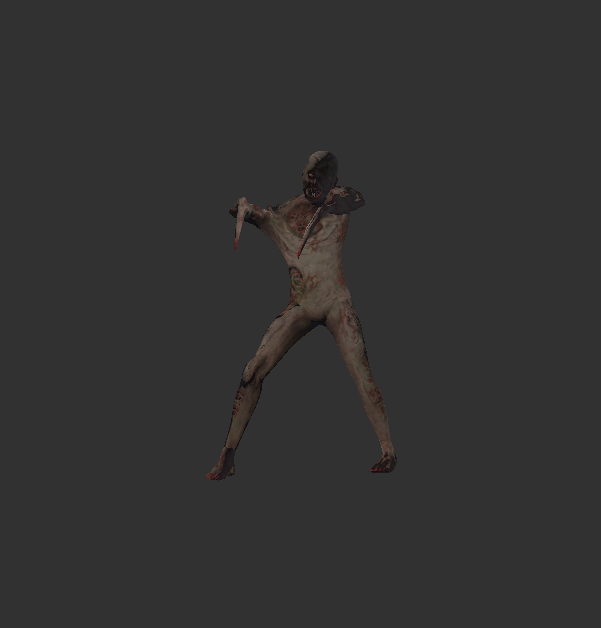
\includegraphics[width=0.8\textwidth]{Reaver.png}
        \caption{Reaver: Standard enemy}
        \label{fig:reaver}
    \end{figure}

    \subsection{Player Animation States}
    \label{appendix:player-animation}

    The player character utilizes a state-based animation system with smooth transitions between key states. Figure \ref{fig:player-states} shows the primary animation states and their transitions.

    \begin{figure}[h]
        \centering
        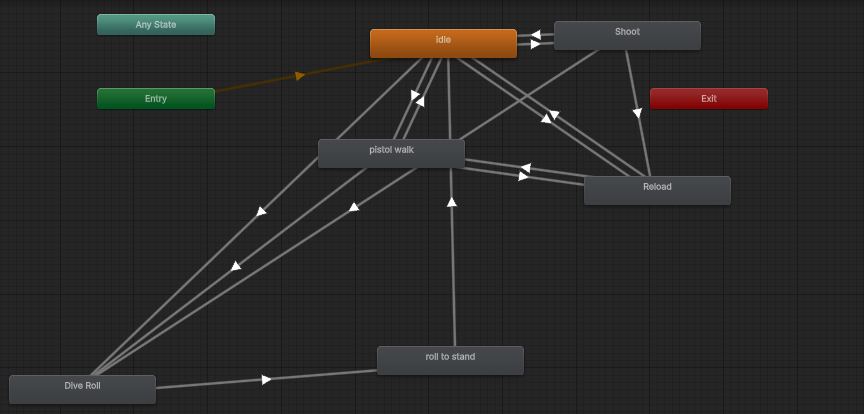
\includegraphics[width=1.2\textwidth]{PlayerState.png}
        \caption{Player Animation State Machine}
        \label{fig:player-states}
    \end{figure}

    The animation system uses boolean parameters and triggers in the Unity Animator to control transitions between states. The core animation states are:

    \begin{itemize}
        \item \textbf{Idle}: Default state when no input is detected
        \item \textbf{Run}: Active when movement input is detected
        \item \textbf{Shoot}: Triggered by left mouse button
        \item \textbf{Reload}: Activated by pressing R key
        \item \textbf{Jump/Dive}: Special movement states with jump triggered by space bar, and dive by pressing space again during the jump window
    \end{itemize}

    The animation controller works in concert with the player controller script to ensure visual feedback matches player input and game state. Transitions between states are managed through a combination of direct trigger calls and continuous parameter updates. The system is designed to handle animation blending for smooth transitions, particularly when changing from movement to combat actions and back.

    The dive roll animation is particuis larly important as it represents both a visual spectacle and a gameplay mechanic, providing brief invulnerability frames that skilled players can use to avoid damage. The reload animation similarly impacts gameplay by preventing other actions during its duration, creating tactical decisions around when to reload.

    \bibliographystyle{alpha}
    \bibliography{sample}

\end{document}